%!TEX program = lualatex

\documentclass[fleqn]{beamer}
\usetheme{metropolis}
\usepackage{graphicx}
\usepackage{comment}
\usepackage{color}
\usepackage{algpseudocode,algorithm}
\usepackage{minted}
\usepackage{listings}
\usepackage{fontspec}
\usepackage{polyglossia}
\setmainlanguage{german}
\usepackage[super]{nth}
\title{Spielekonsole B}
\date{\today}
\author{Robert Schütz, Daniela Kilian, Stefan Müller}
\subtitle{Fortgeschrittenenpraktikum SS 2017}


\begin{document}
	\maketitle
	
	\begin{frame}{Die Crew}
		\setbeamertemplate{section in toc}[sections numbered]
		 \begin{center}
            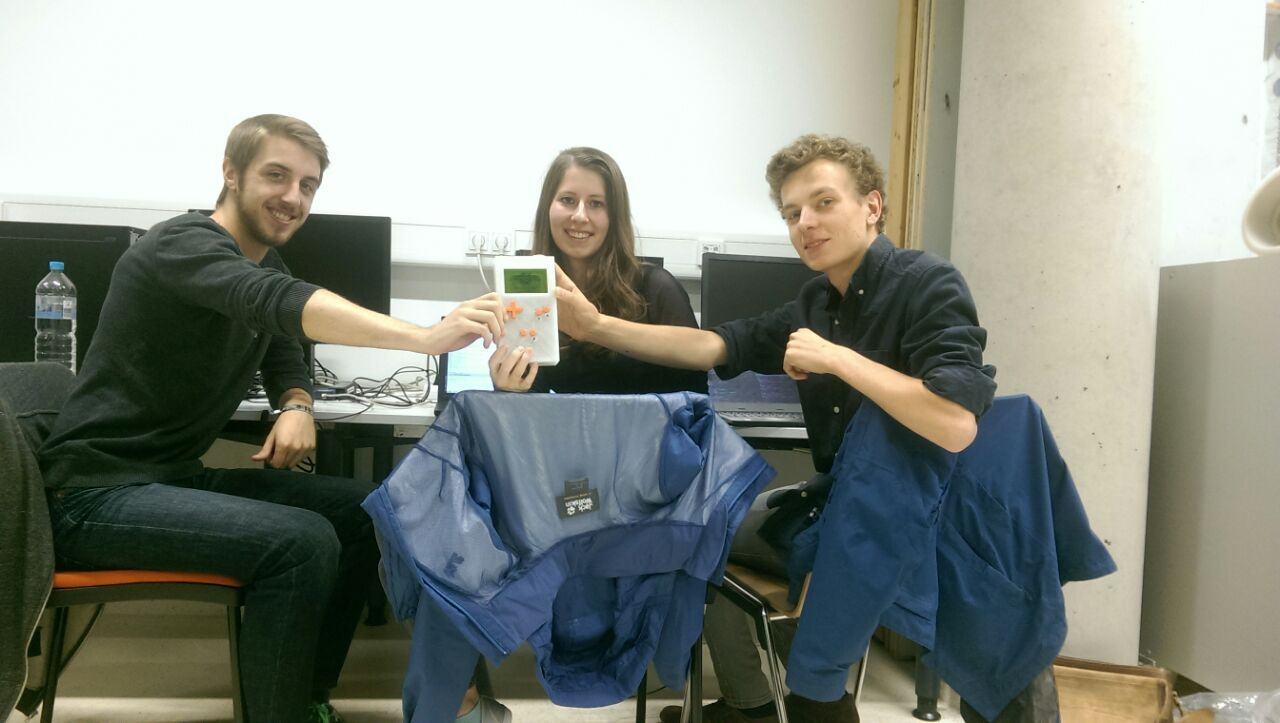
\includegraphics[width=10cm]{Bilder/wir.jpg}
        \end{center}
        \begin{minipage}{0.3\textwidth}
            \centering Stefan Müller
        \end{minipage}
        \begin{minipage}{0.3\textwidth}
            \centering Daniela Kilian
        \end{minipage}
        \begin{minipage}{0.3\textwidth}
            \centering Robert Schütz
        \end{minipage}           
	\end{frame}
    \section{Spielidee}
    \begin{frame}{Das Spiel: Metro HD}
        \begin{center}
            
\includegraphics[width=10cm]{Bilder/splash.png}
        \end{center}
    \end{frame}

    \begin{frame}{Spielaufbau: Schritt 1}
        \begin{center}
            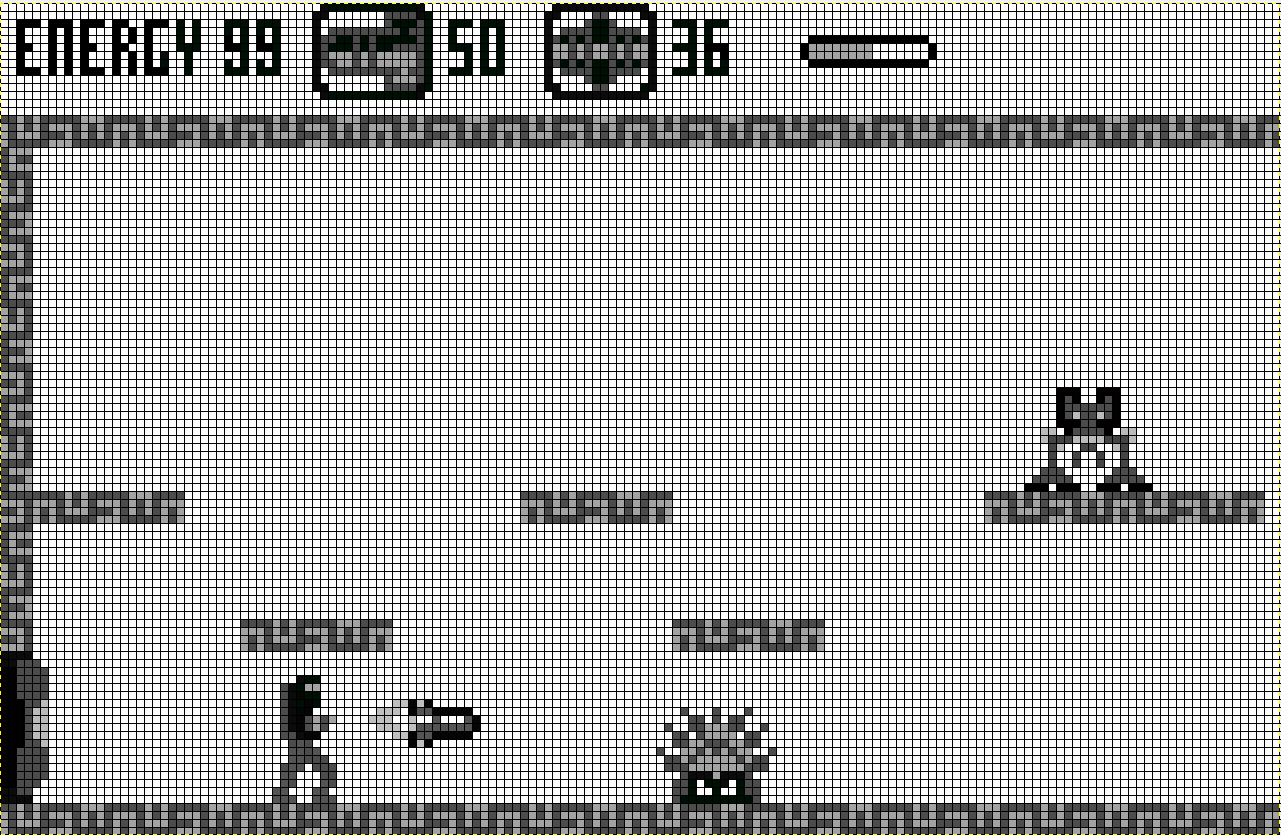
\includegraphics[width=9cm]{Bilder/world2.png}
            
            \large \textbf{Kämpfe gegen verschiedene Monster!}
        \end{center}
     \end{frame}  
    \begin{frame}{Spielaufbau: Schritt 2}
        \begin{center}
            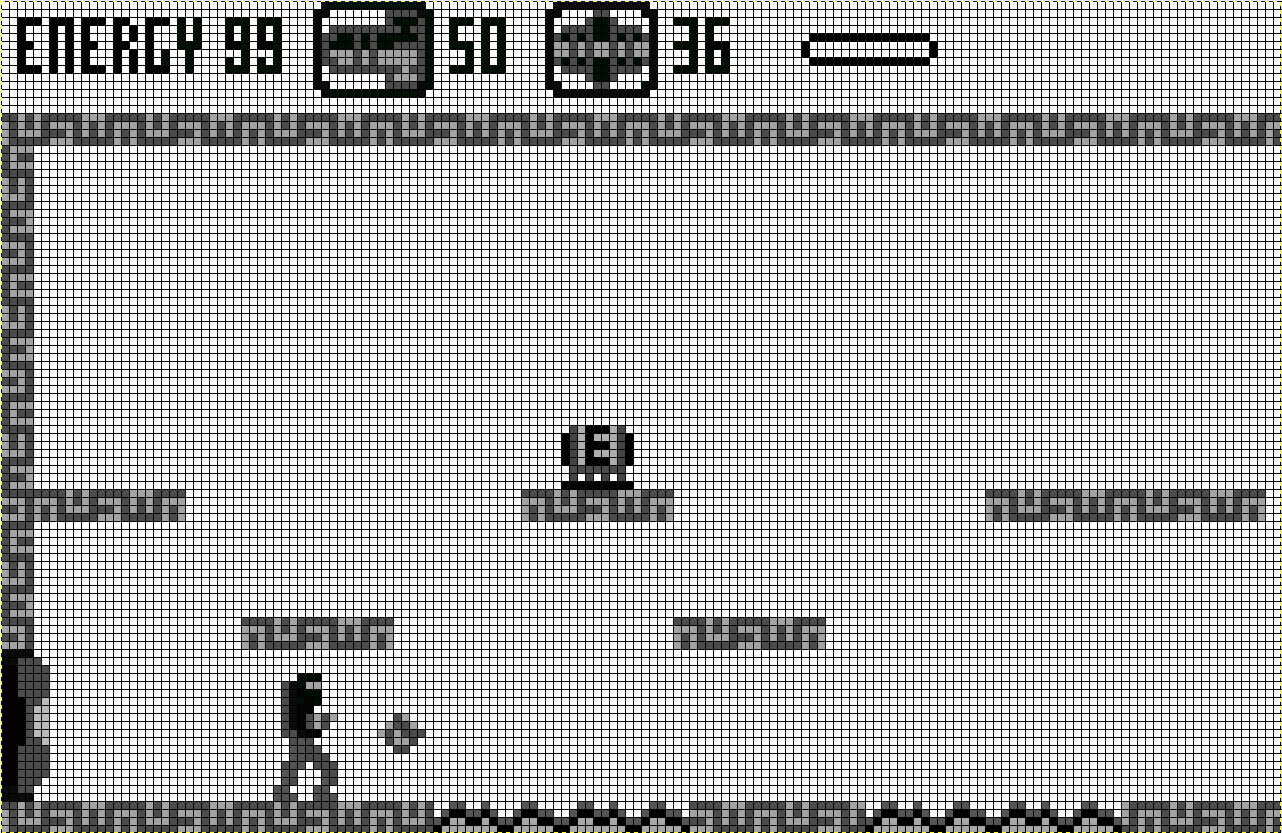
\includegraphics[width=9cm]{Bilder/world3.png}
            
            \large \textbf{Entdecke aufregende Level!}
        \end{center}
    \end{frame}
    \begin{frame}{Spielaufbau: Schritt 3}
        \begin{center}
            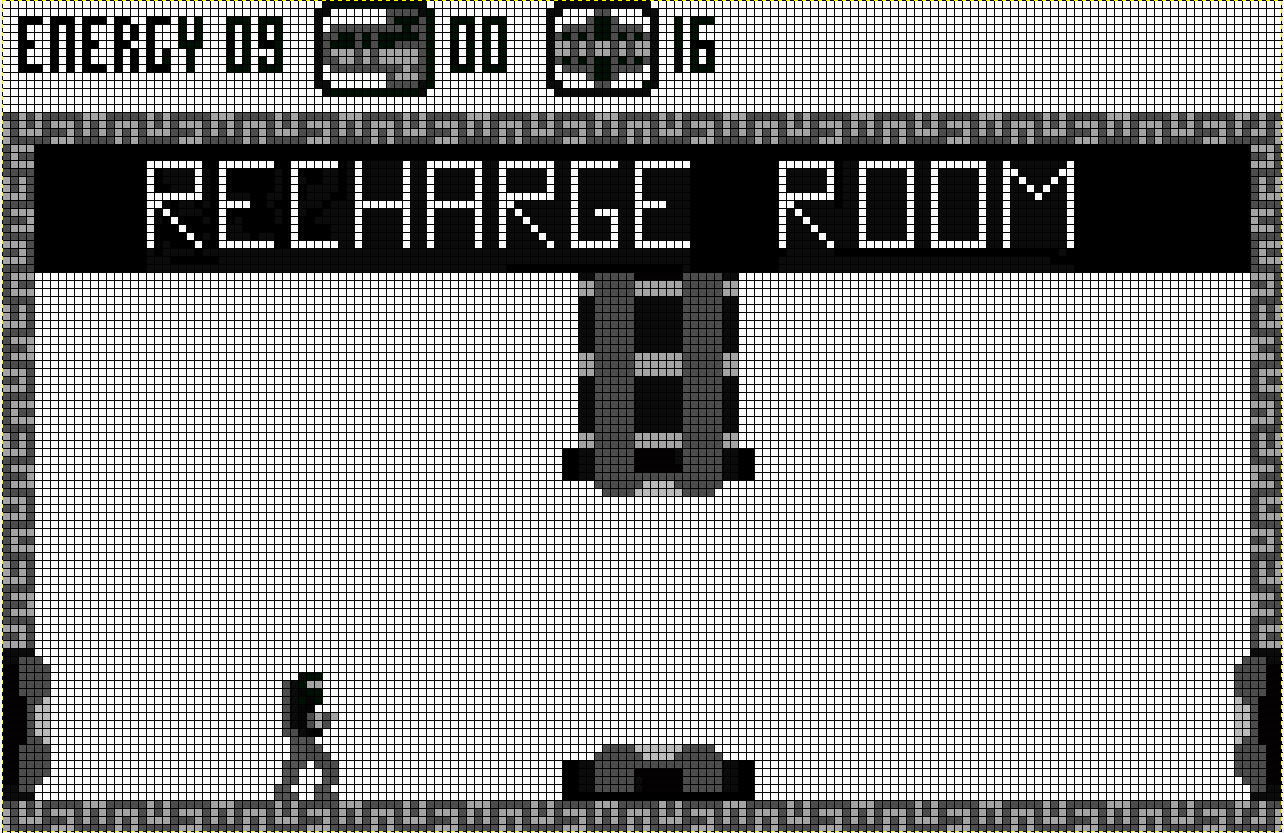
\includegraphics[width=9cm]{Bilder/world4.png}
            
            \large \textbf{Bereite dich auf einen anstrengenden Kampf vor!}
        \end{center}
    \end{frame}
    \begin{frame}{Spielaufbau: Schritt 4}
        \begin{center}
            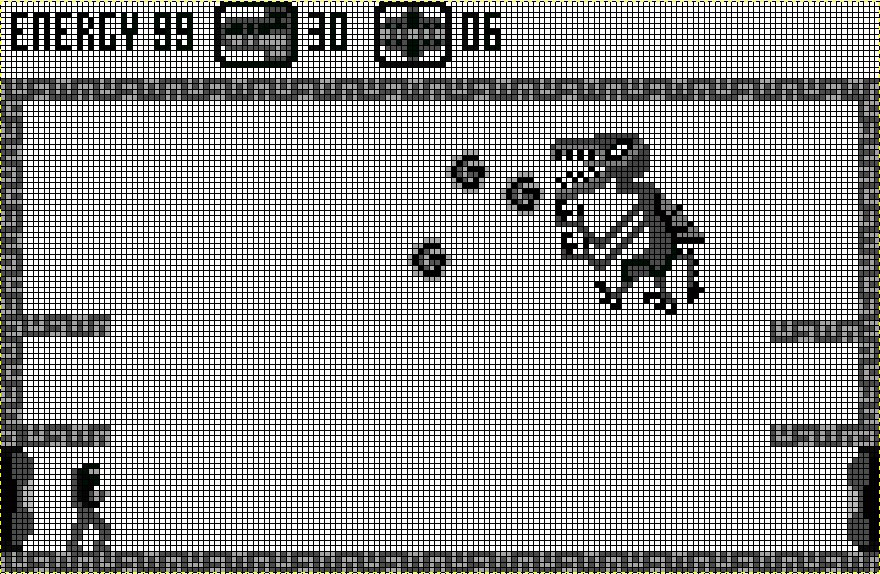
\includegraphics[width=9cm]{Bilder/world6.png}
            
            \large \textbf{Stelle dich gefährlichen Endbossen!}
        \end{center}
    \end{frame}
    \begin{frame}{Spielaufbau: Schritt 5}
        \begin{center}
            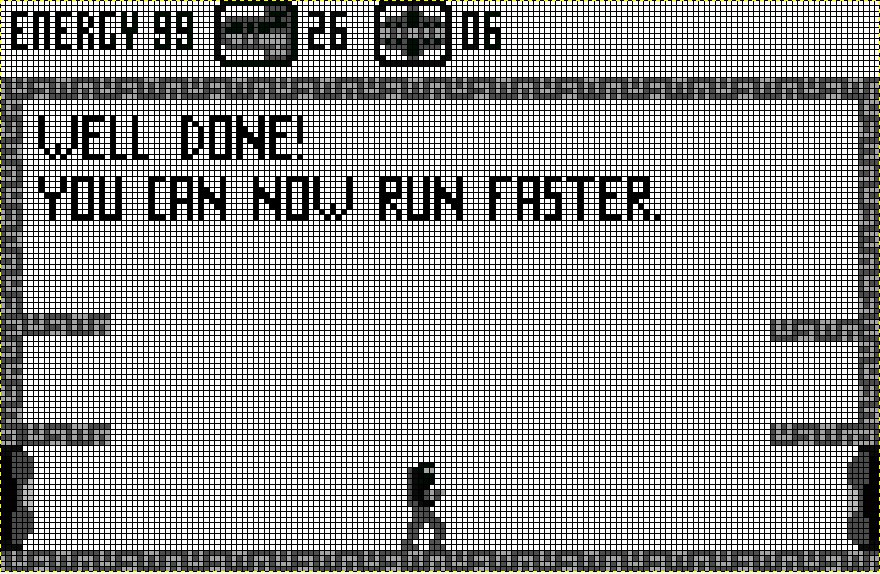
\includegraphics[width=9cm]{Bilder/world5.png}
            
            \large \textbf{Verdiene dir mächtige Power-Ups!}
        \end{center}
    \end{frame}

    \section{Spielumsetzung}
    
    \begin{frame}[fragile]{Zeichen: Sprites}
    Das Display zeichnet immer vier Pixel untereinander auf einmal.
    Ein Python-Skript vereinfacht das Zeichnen:
    
    \begin{minipage}{0.2\textwidth}
        
\includegraphics[width=\textwidth]{Bilder/little.png}
    \end{minipage}
    \begin{minipage}{0.15\textwidth}
        \centering\huge$\longrightarrow$
    \end{minipage}
    \begin{minipage}{0.6\textwidth}
        \small
        \begin{lstlisting}[language=C]
const PROGMEM uint8_t little[16] = {
    0b00000100, 0b00010100,
    0b10010000, 0b10000000,
    0b10000000, 0b10010000,
    0b00010100, 0b00000100, 
    0b00000000, 0b00001000,
    0b11111010, 0b01111001,
    0b01111001, 0b11111010,
    0b00001000, 0b00000000
};
        \end{lstlisting}
    \end{minipage}
    \end{frame}

    \begin{frame}[fragile]{Zeichnen: Display}
    Idee: Window-Funktionalität des Displays benutzen
    
    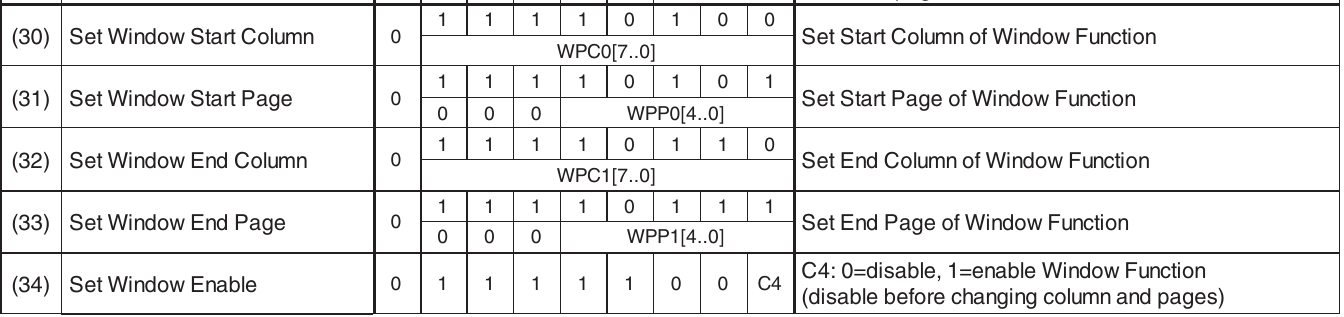
\includegraphics[width=11cm]{Bilder/windowcommands.png}
    
    \begin{minted}[fontsize=\tiny]{C}
void drawsprite(uint8_t x, uint8_t y, uint8_t width, uint8_t height, uint8_t* sprite)
{
    enable_window(x, y, width, height);
    for (uint16_t i = 0; i < width * height; ++i)
        sendbyte(pgm_read_byte_near(sprite + i), 1);
    disable_window();
}     
    \end{minted}
    $\Rightarrow$ Schneller als \mintinline{C}{page()}
    \end{frame}

    \begin{frame}[fragile]{Zeichnen: Pixelweise}
    \begin{minted}[fontsize=\tiny]{C}
void drawsprite_px(uint8_t x, uint8_t y, uint8_t width, uint8_t height, uint8_t* sprite)
{
    uint8_t offset = 2 * (y % 4);
    if (offset == 0)
    {
        drawsprite(x, y / 4, width, height / 4, sprite);
    }
    else
    {
        enable_window(x, y / 4, width, height / 4 + 1);
        uint16_t i = 0;
        for (; i < width; ++i)
            sendbyte(pgm_read_byte_near(sprite + i) << offset, 1);
        for (; i < height / 4 * width; ++i)
            sendbyte(pgm_read_byte_near(sprite + i) << offset | 
                     pgm_read_byte_near(sprite + i - width) >> (8 - offset), 1);
        for (; i < (height / 4 + 1) * width; ++i)
            sendbyte(pgm_read_byte_near(sprite + i - width) >> (8 - offset), 1);
        disable_window();
    }
}   
    \end{minted}
    \end{frame}

    \begin{frame}[fragile]{\mintinline{C}{struct Character}}
Alle beweglichen Objekte werden als \mintinline{C}{Character} repräsentiert.
\begin{minted}[fontsize=\tiny]{C}
struct Character
{
    uint8_t x;
    uint8_t y;
    enum {LOOK_MONSTER_MEMU, LOOK_PROTAGONIST, LOOK_FIREBALL, ...} look;
    uint8_t lookstate; // to e.g. store whether the wings are turned upwards or downwards
    uint32_t lastlookstatechg;
    uint8_t width;  // in pixels
    uint8_t height; // in pixels
    enum {DIRECTION_LEFT, DIRECTION_RIGHT} direction;
    enum {DIRECTION_UP, DIRECTION_DOWN} verticaldirection;
    int8_t jumpstate;
    uint8_t initial_health;
    int8_t health;
    uint8_t damage;
    uint8_t jumpheight;
    enum {FOLLOW_PROTAGONIST, BACK_AND_FORTH, ...} movement;
    uint8_t x_pace;
    uint8_t y_pace;
};
\end{minted}
\end{frame}
    
    \begin{frame}[fragile]{Spielablauf}
    \begin{minted}[fontsize=\tiny]{C}
while(1)
{
    if (nextmoveevent < getMsTimer())
    {
        if (B_RIGHT)
        {
            moveright(protagonist);
            nextmoveevent = getMsTimer() + 50;
        }
        ...
    }
    if (projectile->movement == HIDDEN
        && num_rockets > 0
        && nextshootevent < getMsTimer()
        && B_A)
    {
        projectile->movement = PROJECTILE;
        draw(projectile);
        num_rockets--;
        eeprom_write_byte(&num_rockets_stored, num_rockets);
        nextshootevent = getMsTimer() + 500;
    }
    if (monster->movement != HIDDEN && collision(protagonist, monster))
    {
        takingdamage(monster->damage);
    }
    ...
}    
    \end{minted}
    \end{frame}
    
        \begin{frame}[fragile]{Zufällige Plattformen}
    \begin{minted}[fontsize=\tiny]{C}
srandom(level_seed + level_pos);    
platforms_13 = random();
platforms_19 = random();
platforms_24 = random();   
nofloor = random();

bool obstacle(uint8_t x, uint8_t y)
{
    if (y >= 19 * 4 && y < 20 * 4)
        return !(platforms_19 & (3l << (x / PLATFORM_WIDTH * 2)));
    else if (y >= 13 * 4 && y < 14 * 4)
        return !(platforms_13 & (3l << (x / PLATFORM_WIDTH * 2)));
    else if (y >= 24 * 4 && y < 25 * 4)
        return !(platforms_24 & (3l << (x / 16 * 2)));
    else if (y >= FLOOR_Y && y < FLOOR_Y + 4)
        return nofloor & (3l << x / 16 * 2);
    else
        return false;
}
    \end{minted}
    Die \mintinline{C}{obstacle()} Funktion dient dazu, herauszufinden, ob an einer gegebenen Stelle eine Plattform ist.
    \end{frame}
    
    \begin{frame}{Tiefensuche: Schritt 1}
    		\begin{center}
    			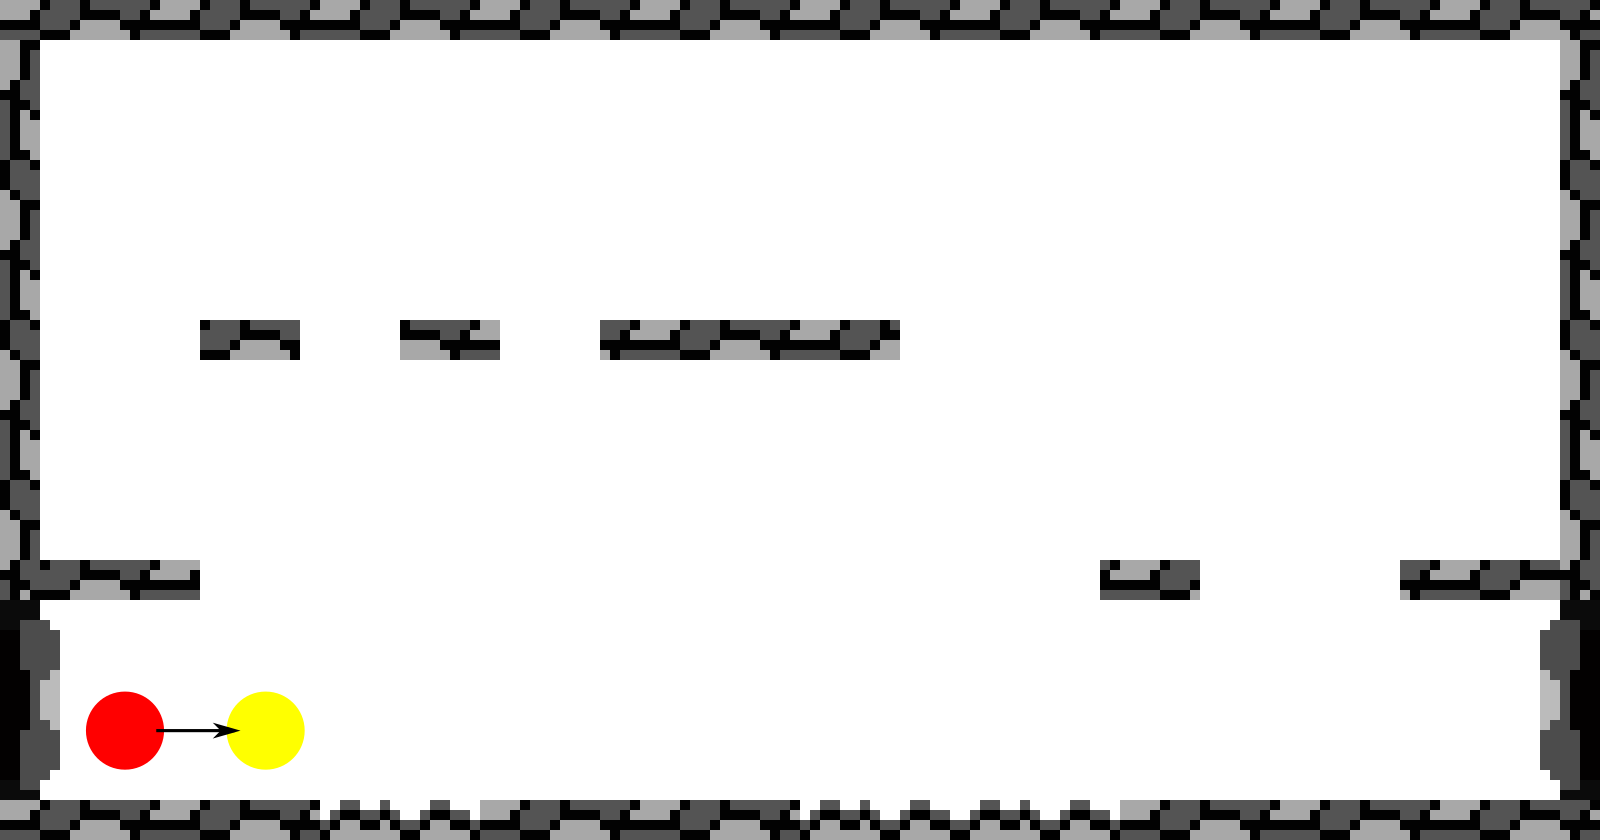
\includegraphics[width=11cm]{Bilder/dfs1.png}
    		\end{center}
    \end{frame}
    
    \begin{frame}{Tiefensuche: Schritt 2}
    		\begin{center}
    			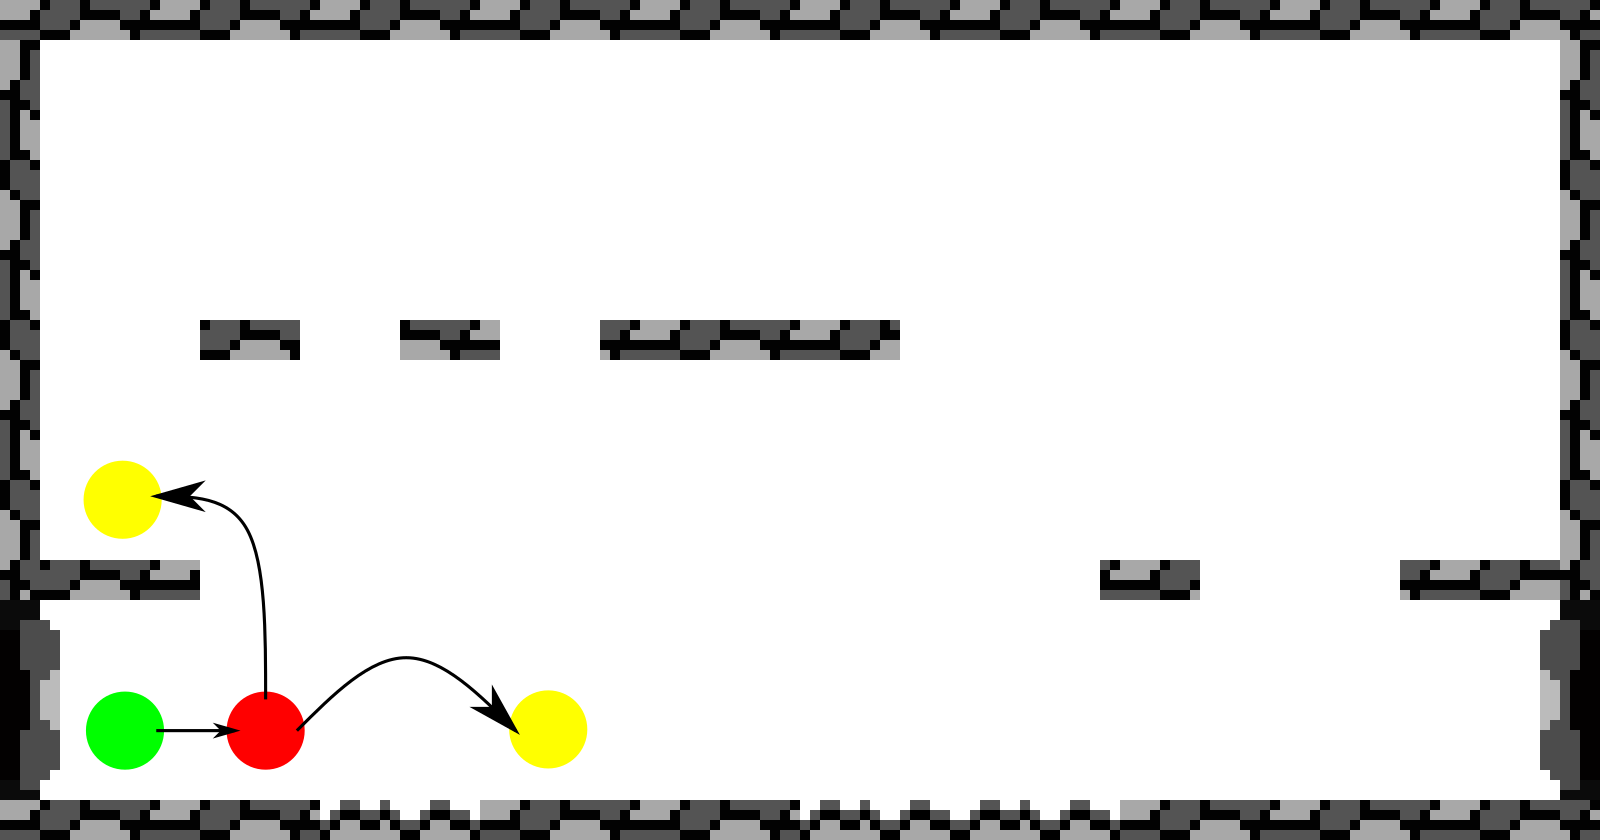
\includegraphics[width=11cm]{Bilder/dfs2.png}
    		\end{center}
    \end{frame}
    
    \begin{frame}{Tiefensuche: Schritt 3}
    		\begin{center}
    			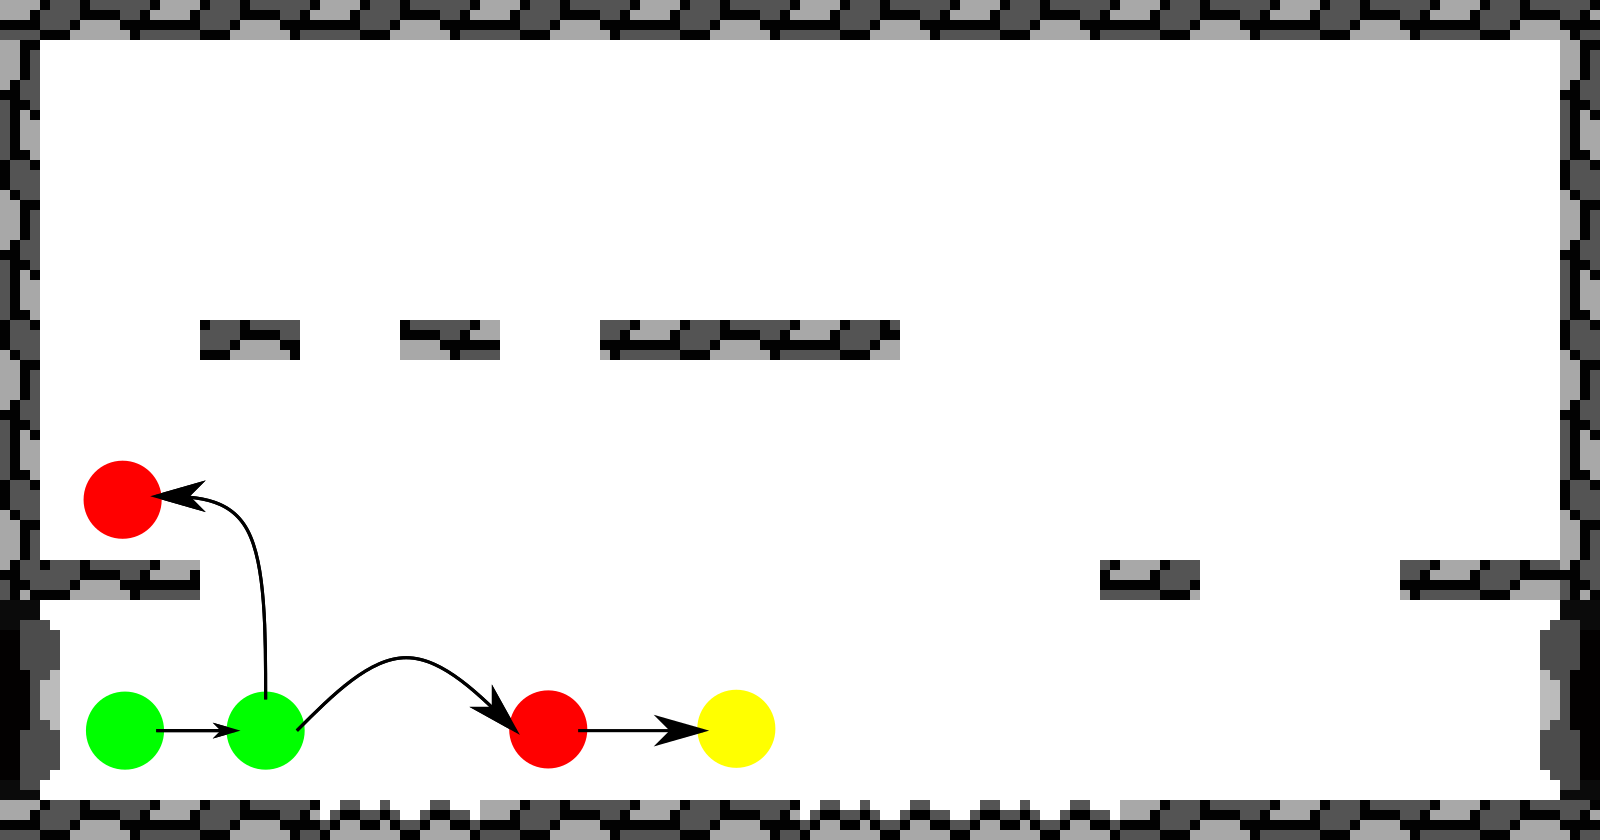
\includegraphics[width=11cm]{Bilder/dfs3.png}
    		\end{center}
    \end{frame}
    
    \begin{frame}{Tiefensuche: Schritt 4}
    		\begin{center}
    			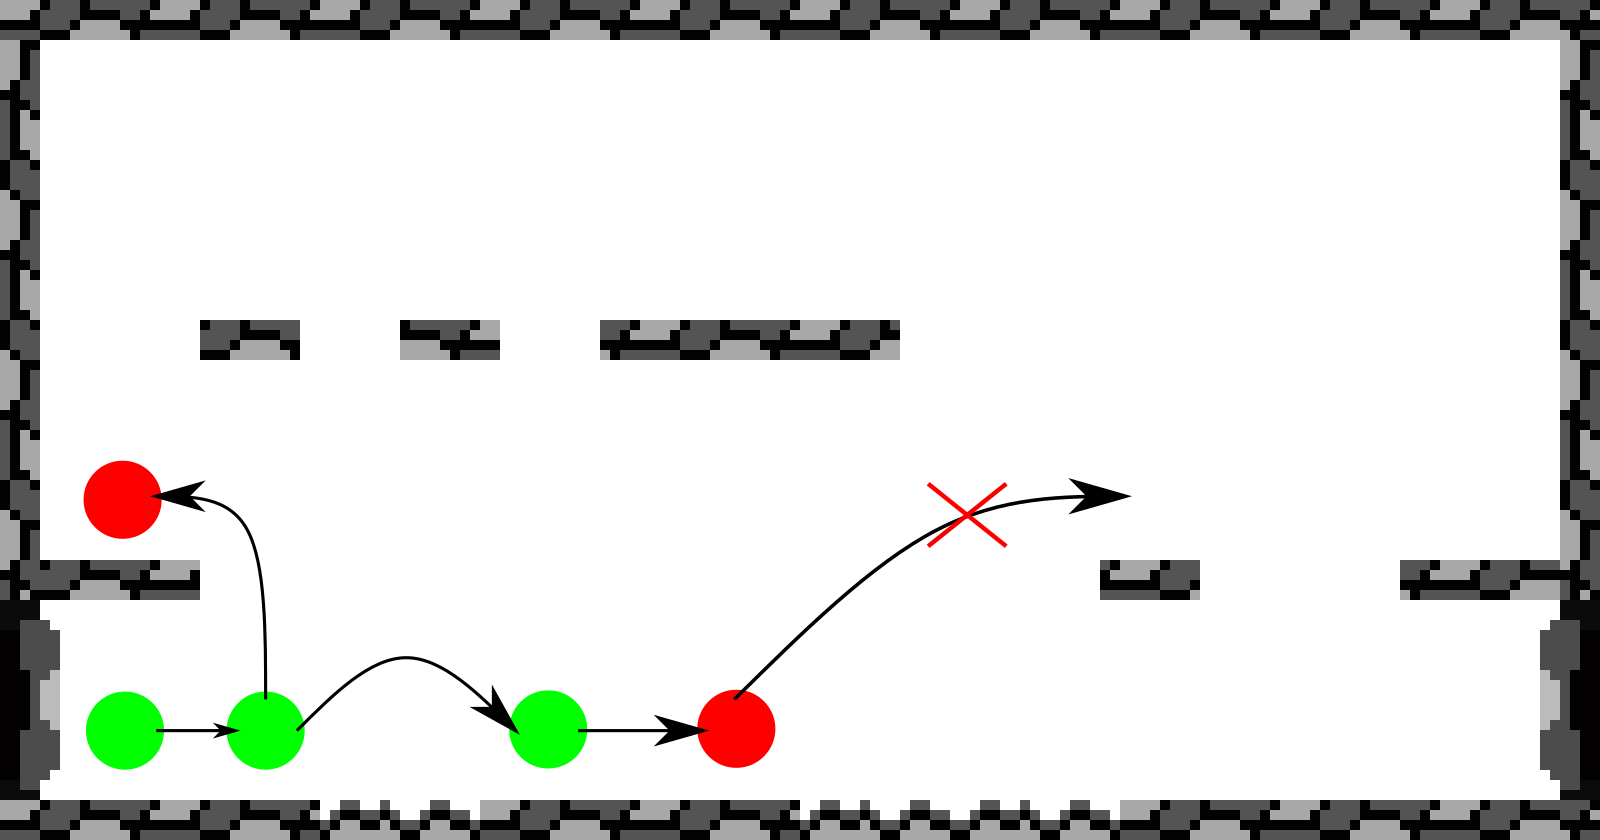
\includegraphics[width=11cm]{Bilder/dfs4.png}
    		\end{center}
    \end{frame}
	\begin{frame}{Tiefensuche: Schritt 5}
    		\begin{center}
    			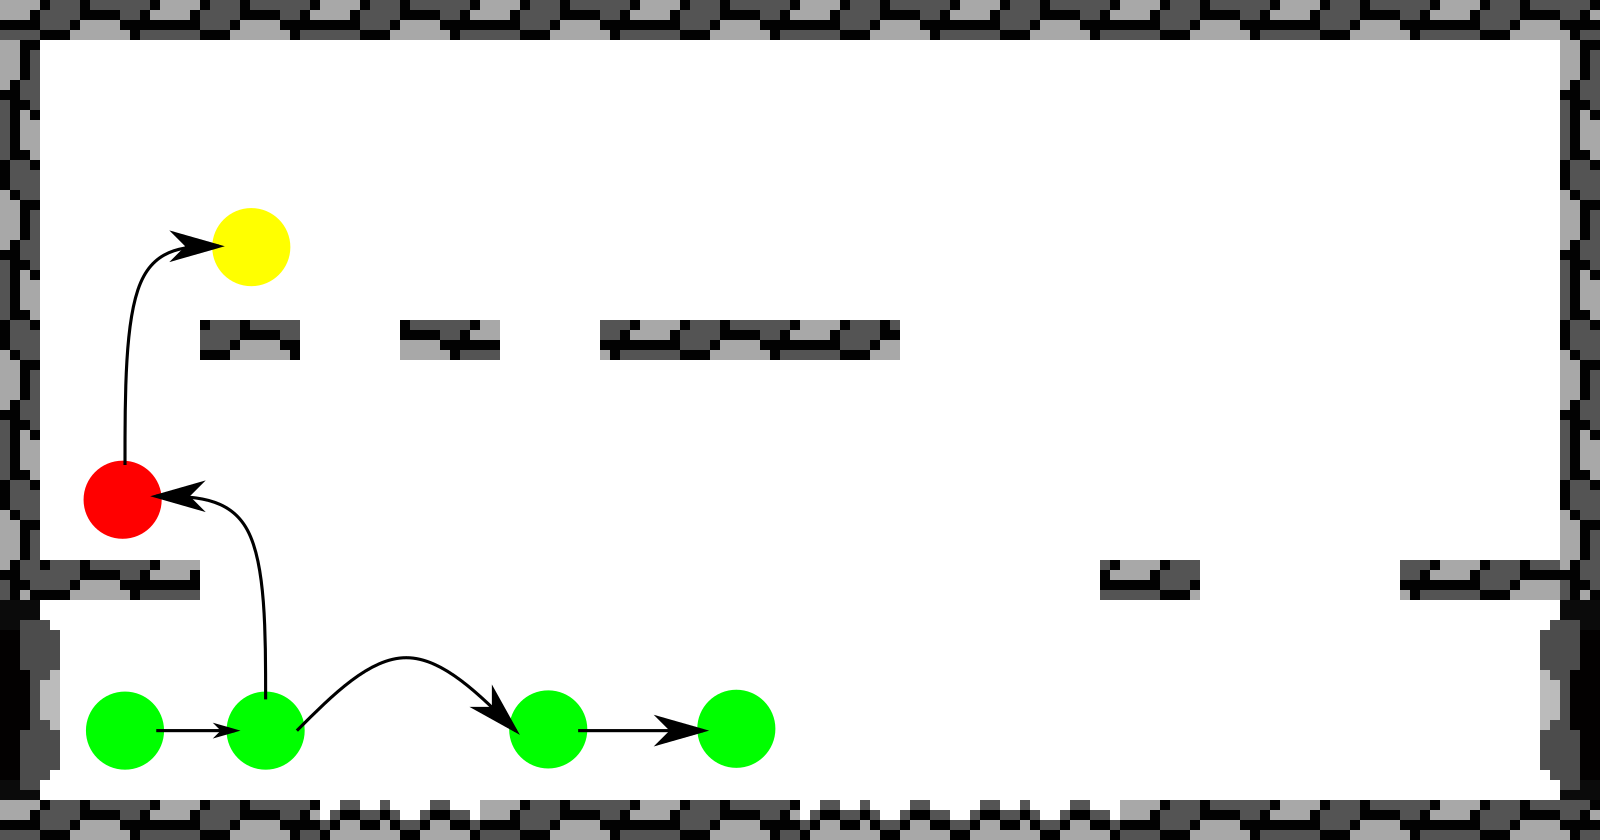
\includegraphics[width=11cm]{Bilder/dfs5.png}
    		\end{center}
    \end{frame}  
    \begin{frame}{Tiefensuche: Schritt 6}
    		\begin{center}
    			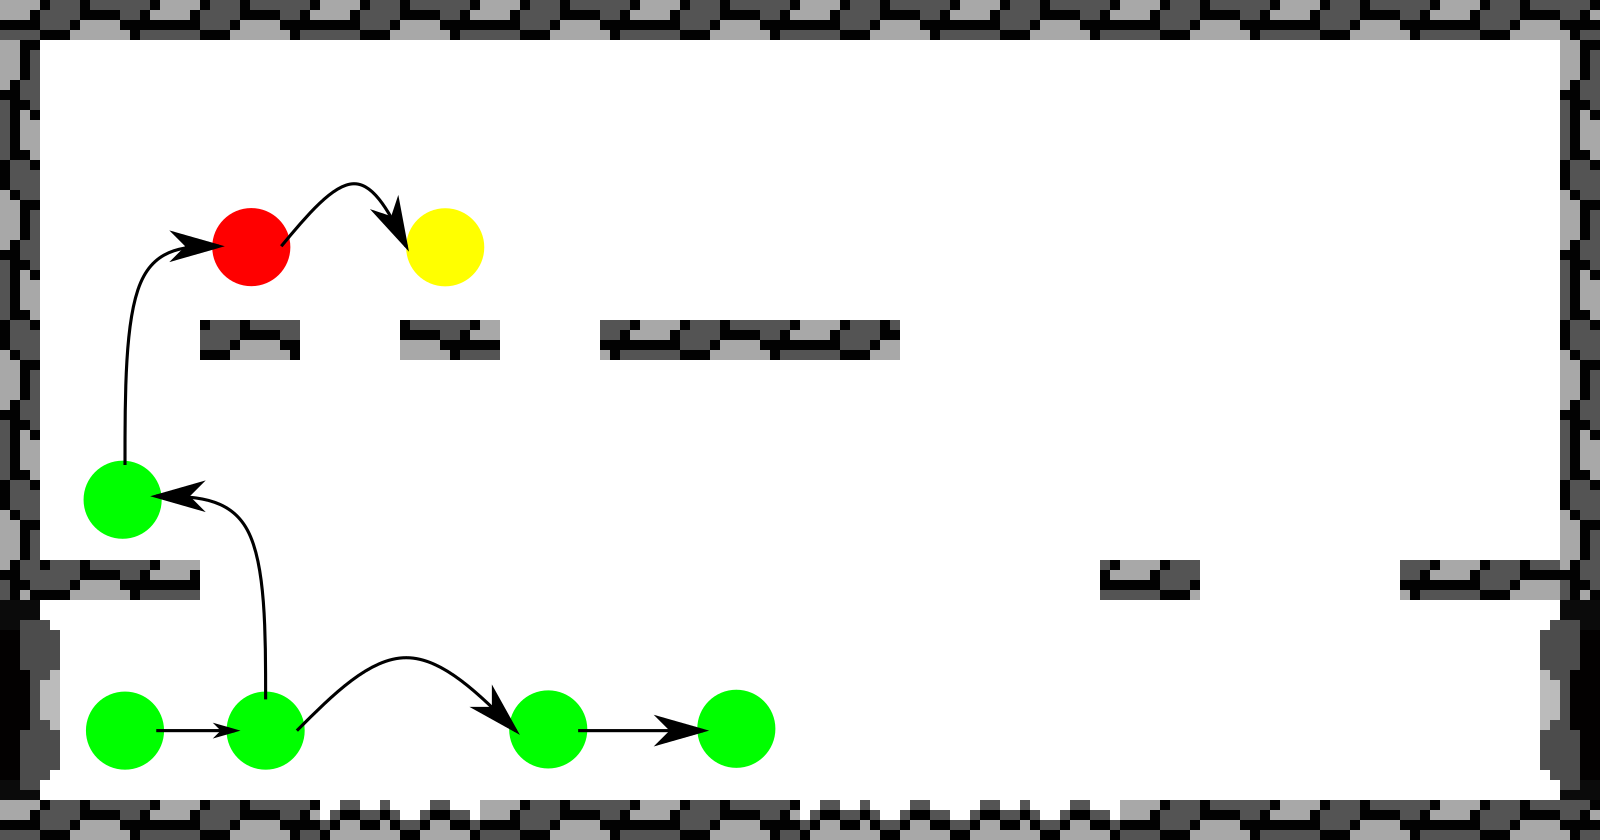
\includegraphics[width=11cm]{Bilder/dfs6.png}
    		\end{center}
    \end{frame}
    \begin{frame}{Tiefensuche: Letzter Schritt}
    		\begin{center}
    			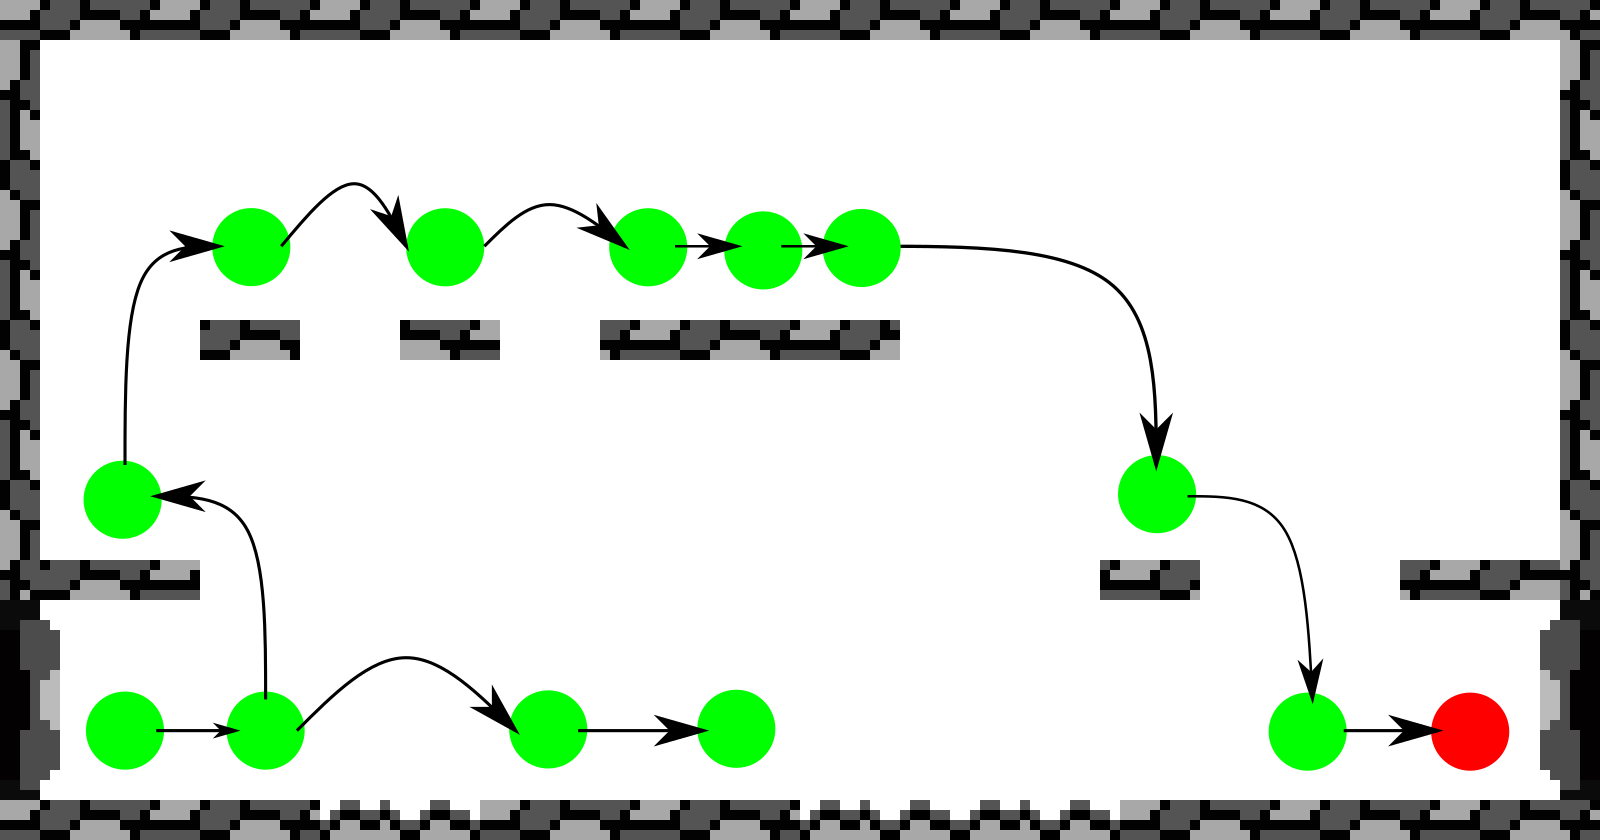
\includegraphics[width=11cm]{Bilder/dfs7.png}
    		\end{center}
    \end{frame}    
    
    \section{Sound}
    \begin{frame}{Timer}
    Wir verwenden zwei Timer:
    \begin{itemize}
	    \item Timer1
	    		\begin{itemize}
	    			\item Frequenz: 62\,500 Hz
	    			\item Toggelt Pin B1
	    			\item Pulsweite bestimmt „Ausschlag“ der Welle
	    			
	    		\end{itemize}
    \end{itemize}
    \begin{center}
    		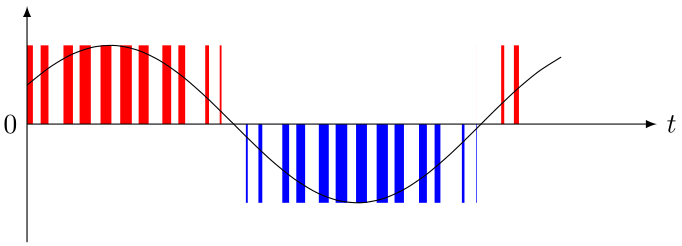
\includegraphics[width=8cm]{Bilder/pwm}
    \end{center}
    \end{frame}
    
    \begin{frame}{Timer}
    		\begin{itemize}
    			\item Timer2
	    		\begin{itemize}
	    			\item Frequenz des Interrupts: 15\,625 Hz
	    			\item Dient zur Zeitmessung
	    			\item Legt den aktuellen Ausschlag fest:
	    				
	    				Für einen Ton mit 440 Hz wird bei jedem Aufruf des Interrupts die Pulsweite (max.\ 255) um 
	    				\[255 / (15625/440) \approx 7,18\]
	    				erhöht. 
	    				Für eine höhere Genauigkeit werden \mintinline{C}{uint16_t}s verwendet.
	    		\end{itemize}
    		\end{itemize}
    		
    \end{frame}
    
    \begin{frame}[fragile]{MIDI einlesen}
    \begin{center}
        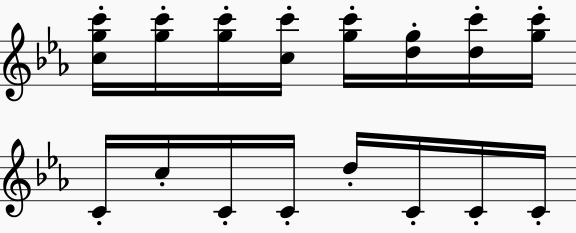
\includegraphics[height=2cm]{Bilder/noten.png}
        
        \huge$\downarrow$
        
        \begin{minted}[fontsize=\small]{C}
const Event boss4[] PROGMEM = {
  { { .track = 0, .increment = 615, .delay = 0 } },
  { { .track = 1, .increment = 307, .delay = 0 } },
  { { .track = 2, .increment = 2463, .delay = 2812 } },
  { { .track = 2, .increment = 1231, .delay = 2812 } },
  { { .track = 0, .increment = 1231, .delay = 0 } },
  ...,
  STOP
};
        \end{minted}
    \end{center}
    \end{frame}

\section{Probleme und Verbesserungen}
    \begin{frame}{Aufgetretene Probleme}
        \begin{itemize}
            \item Problem: Speicherplatzmangel
        \end{itemize}
        \begin{center}
            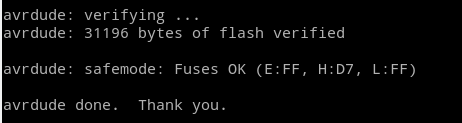
\includegraphics[width=7cm]{Bilder/speicherplatz.png}
        \end{center}
        \begin{itemize}
            \item Lösung: Ablegen der Sprites im PROGMEM und
            effiziente Aufspaltung von großen Bildern
        \end{itemize}
        \begin{center}
           % 
\includegraphics[height=2cm]{Bilder/splashleft.png}
           % 
\includegraphics[height=3cm]{Bilder/splashcenter.png}
           % 
\includegraphics[height=2cm]{Bilder/splashright.png}
           
\includegraphics[width=6cm, height=3cm]{Bilder/splashspeicher.png}
        \end{center}
    \end{frame}


    \begin{frame}{Mögliche Verbesserungen}
    Hardware
    		\begin{itemize}
    		\item Tiefpass einbauen
    		\item Farbdisplay
    		\end{itemize}
    		
    Software
        \begin{itemize}
        		\item (Noch) Effizientere Implementierung 
            \item Highscore hinzufügen
            \item Spiel weiter ausbauen:
                \begin{itemize}
                    \item Neue Monster, Endbosse und Power-Ups
                    \item Weitere Waffen
                    \item Geheimwege
                \end{itemize}
            
        \end{itemize}
    \end{frame}
    

    \begin{frame}
    		
\includegraphics[width=11cm]{Bilder/aufmerksamkeit.png}
    \end{frame}
   
\end{document}
